\chapter{Motivation}\label{ch:motivation}

The rapid growth of urban populations and the corresponding increase in vehicle ownership have significantly intensified the challenges associated with parking management in cities worldwide. For instance, the dramatic rise in car usage in Madrid has substantially contributed to heightened levels of environmental pollution \autocite{environmental_impact_madrid_central}. Despite the number of parking spaces in Spain remaining stable between 2014 and 2020 \autocite{urban_mobility_trends}, the escalating demand for parking has resulted in higher costs, prolonged search times, increased traffic congestion, and elevated urban pollution levels.

The inadequacies of traditional, manual Parking Management Systems (PMSs) have further highlighted the need for innovative solutions in this domain. Studies highlight the importance of user-friendly, secure, and reliable systems, with these factors playing a crucial role in influencing parking behavior and preferences. This growing demand for smart parking solutions is reflected in the global market projections, which show remarkable growth from \$7.11 billion (US) in 2023 to an expected \$18.13 billion (US) by 2028, with a \gls{cagr} of 20.2\% \autocite{smart_parking_system_market_report_2024}, see \cref{fig:smart_parking_system_market_report_2024}.

\begin{figure}
	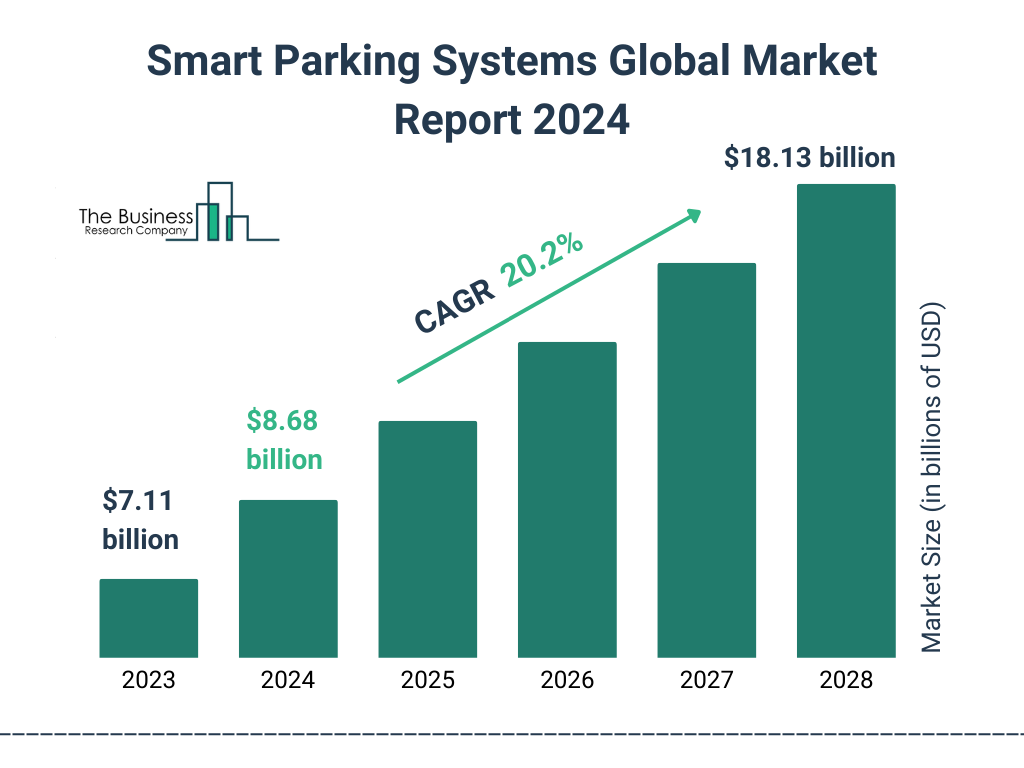
\includegraphics{smart_parking_system_market_report_2024.png}
	\caption{Smart Parking System Market Report 2024 \autocite{smart_parking_system_market_report_2024}}\label{fig:smart_parking_system_market_report_2024}
\end{figure}

Advancements in technology provide new opportunities to address these challenges. The proliferation of internet-connected devices, growing by 20\% annually \autocite{iot_growth}, has catalyzed the emergence of \gls{iot}-based \glspl{pms}. These systems aim to mitigate traffic congestion and reduce urban pollution while promoting sustainable and efficient urban mobility. By leveraging real-time data and automation, modern \glspl{pms} offer transformative potential for urban planning and management.

Integrating these advanced systems into urban environments offers multiple benefits, including decreased traffic congestion, reduced pollution, enhanced security, and an improved quality of life for residents. Additionally, \glspl{pms} enable automated parking space management, making them adaptable for a wide range of applications, including urban centers, residential communities, and commercial buildings.

Despite these advancements, the widespread adoption of \glspl{pms} in Spain has faced significant obstacles. Many existing systems rely heavily on human intervention, leading to delays, insufficient information dissemination, and limited control over parking space availability. This dependence on manual operations not only impairs system efficiency but also increases operational costs.

Emerging technologies have inspired the development of innovative \glspl{pms}, such as RFID-based systems \autocite{rfid_smart_parking_management_system}, \gls{iot}-enabled solutions \autocite{development_smart_parking_management_system}, and intelligent parking systems employing image processing techniques \autocite{intelligent_parking_system_image_processing}. However, these systems frequently rely on centralized architectures, which are prone to scalability and reliability issues, particularly during service disruptions. Moreover, many current solutions lack the flexibility needed to accommodate the specific requirements of diverse user groups, limiting their broader applicability.

Addressing these limitations, the primary objective of this project is to design and implement a fully distributed and autonomous \gls{pms} that overcomes the challenges inherent in existing systems. This new approach emphasizes scalability, reliability, and adaptability, with a particular focus on meeting the demands of next-generation smart cities. Through this work, the project aims to contribute to the development of sustainable, efficient, and user-centric parking solutions for urban environments.

